%3.1.tex
LLVMは2000年にイリノイ大学で開発が開始されたコンパイラ基盤である.コンパイラ基盤とはコンパイラに必要となるモジュールをまとめたもので,コンパイラを開発するためのフレームワークである.
LLVMの構成を図\ref{fig:LLVM}に示す.LLVMはソースコードをLLVMの中間表現であるLLVM IRに変換するフロントエンド,LLVM IRに対して最適化等の操作やLLVM IRから機械語やアセンブリコードへの変換を行うバックエンドに分かれている.図\ref{fig:LLVM}の様に,C言語等のソースコードから任意のアーキテクチャのアセンブリコードや機械語コードの生成を行うことができる.
LLVMではこれらの機能がモジュール化されており,新規機能を実装する際に再利用することができる.例えば新たなアーキテクチャ向けのコンパイラを開発する際はバックエンドのみ実装を行い,フロントエンドについては再利用することができる.

\begin{figure}[b]
    \centering
    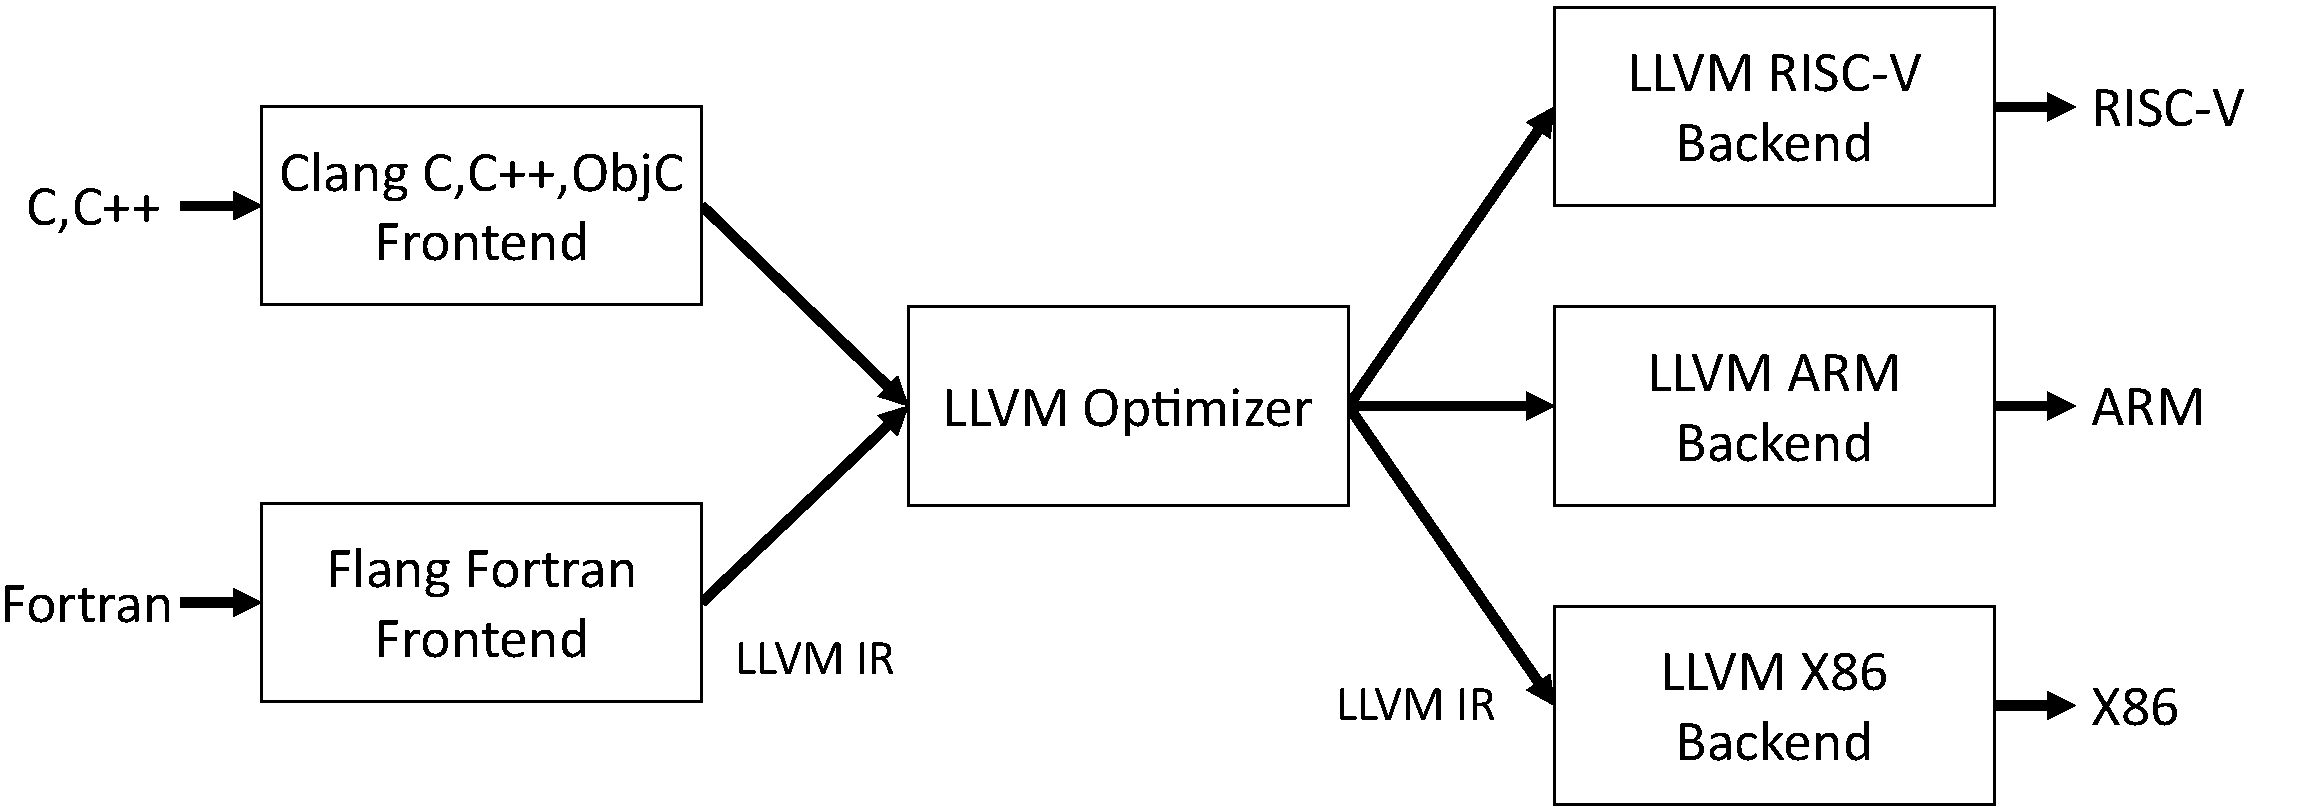
\includegraphics[scale=0.4]{image/LLVM.pdf}
    \caption{LLVMの構成}
    \label{fig:LLVM}
\end{figure}

LLVMには既にRISC-Vを対象としたコード生成のためのバックエンドが実装されている.本研究ではRISC-Vを独自にベクトル拡張したベクトル拡張付きRISC-Vの命令の生成を目的としているため,このRISC-V向けのバックエンドに対して変更を加えることによって独自命令コードの生成を行う.

LLVMバックエンドにおけるコード生成の流れを図\ref{fig:LLVM_backend}に示す.
LLVMバックエンドではPassによって処理が行われる.PassとはLLVMコンパイラにおいて変換や最適化を実行するもので,中間表現に対する変換や最適化等を行う.
図\ref{fig:LLVM_backend}
ではLLVMバックエンドにおけるデータフォーマットの変化と実行されるPassを表している.

\begin{figure}[tb]
    \centering
    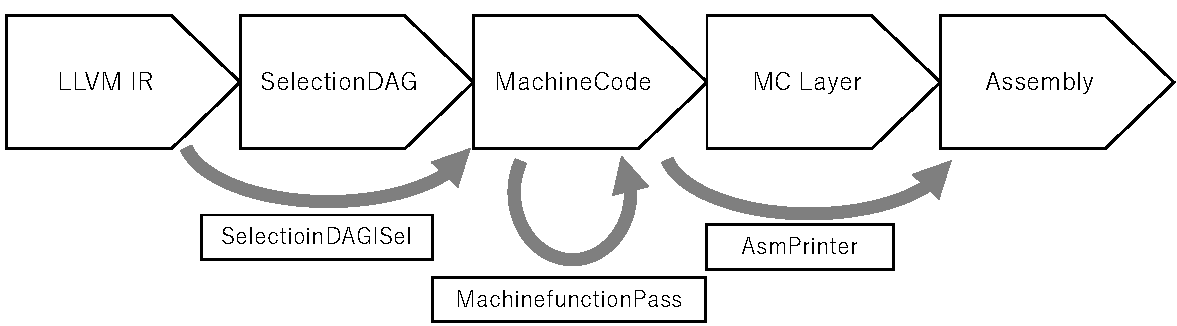
\includegraphics[scale=0.7]{image/backend.pdf}
    \caption{LLVMバックエンド}
    \label{fig:LLVM_backend}
\end{figure}

バックエンドではLLVM IRからDAG (Directed Acyclic Graph)であるSelectionDAGへフォーマットを変換する.SelectionDAGはLLVM IRをグラフ形式で表したもので,各命令やデータの依存関係を表現する.LLVMにおけるSelectionDAGを図\ref{fig:dag}に示す.図\ref{fig:dag}のSelectionDAGは2変数を加算し,その結果を返す関数のSelectionDAGである.CopyFromRegノードはレジスタから値を取得するノードであり,2つのCopyFromRegノードをADDWノードで加算し,レジスタに値を渡すCopyToRegによって加算結果を返す.
SelectionDAGへの変換はSelectionDAGISelパスで行われ,SelectionDAGは最終的にSelectionDAGISelパスによってMachineCod形式に変換される.SelectionDAGISelではLower,Combine,Legalize,Select,Scheduleのフェーズから構成される.

\begin{figure}[tb]
    \centering
    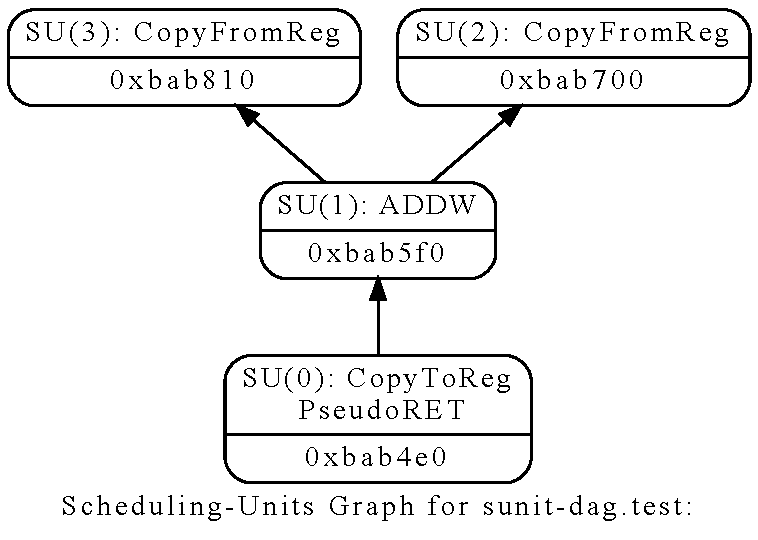
\includegraphics[scale=0.6]{image/dag.pdf}
    \caption{SelectionDAG}
    \label{fig:dag}
\end{figure}

LowerはLLVM IRからSelectionDAGに変化させるフェーズである.このフェーズではLLVM IRからSelectionDAGのノードへと一対一の対応を行う.この段階では生成対象のアーキテクチャであるターゲットマシンでは利用できない命令やデータ形式を含んでる不正 (illegal)な状態である.

Combineフェーズではパターンマッチングによる置き換えで最適化を行い,処理に必要な命令数を削減するなどの命令の単純化を行う.

Legalizeはターゲットマシンではサポートされていない命令やデータ形式を他のものに置き換えるフェーズである.このフェーズによって不正な状態であったSelectionDAGノードがターゲットマシンで利用できない命令やデータ形式が変換され,ターゲットマシンの命令に変換が可能である正当 (legal)な状態となる.

SelectフェーズではこれまでLLVM IRの命令を用いていたSelectionDAGのノードを生成対象のアーキテクチャであるターゲットマシンの命令を用いるMachineNodeへと変換する.

Scheduleフェーズでは構築されたグラフの依存関係を元に命令をスケジューリングし,命令の順序を決定するフェーズである.

SelectionDAGISelパスではこれらのすべてのフェーズが終わった後にMachineCodeを出力する.

MachinefunctionパスではMachineCode形式をアセンブリコードや機械語コードとして出力できる様に物理レジスタの割当て等を行う.MachineCode形式はLLVM IRとは異なり,階層構造がない形式である.MachineCode形式を図\ref{fig:machine_code}に示す.3,4行目にてレジスタから値のコピーを行っており,5行目にて値の加算を行っている.3,4,5行目において変数\%0,\%1,\%2,の末尾にgprとあるが,これは使用するレジスタの種類を指定しており,gprは汎用レジスタを指定している.後述するレジスタの割当はこの指定にしたがって行われる.

\begin{figure}
    \centering
    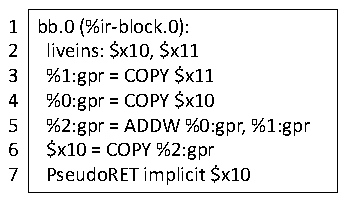
\includegraphics[scale=1.0]{image/machine_code.pdf}
    \caption{MachineCode}
    \label{fig:machine_code}
\end{figure}

MachineCodeがSelectionDAGISelによって生成された直後はまだ命令で扱うレジスタは無限個あると仮定した仮想レジスタやphi命令を含んだSSA (Static Single Assignment form)形式で表現されている.phi命令とは,SSA形式においてどの制御フローから到達したのかによって変数を選択する関数である.phi命令の例を図\ref{fig:phi_func}に示す.図\ref{fig:phi_func}ではL3で使用している変数a3の定義を決定するためにphi命令を用いている.このphi命令ではL1から来たときはa3にa1を代入し,L2から来たときはa3にa2を代入する.これによってSSA形式において変数の定義が一意に決まらない処理を実現している.
MachinefunctionPassでは仮想レジスタから実際にアセンブリコードで用いられる物理レジスタの割当てを行う.また,phi命令は従来の命令セットにおいてphi命令を実装していないためLLVMでは実行可能コード生成のためにphi命令の削除を行い,MachineCodeを非SSA形式へと変換する.

\begin{figure}[tb]
    \centering
    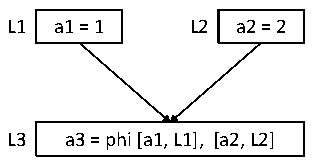
\includegraphics[scale=1.0]{image/phi_function.pdf}
    \caption{SSA形式でのphi命令}
    \label{fig:phi_func}
\end{figure}

AsmPrinterパスはMachineCodeをMC Layer形式へと変換した後にアセンブリコード,オブジェクトファイルを出力するパスである.MC Layer形式はMachineCode形式のような階層構造がない形式である.MC Layer形式では命令とオペランドの情報を持っており,アセンブリコードと出力する際は命令とオペランドに対応する命令ニーモニックを出力する.オブジェクトファイルを出力する際は命令とオペランドの情報をもとに対応する機械語コードを出力する.MC Layer形式の例を図\ref{fig:MCLayer}に示す.MC Layerでは命令を2,6行目のようにMCInstの名称で持っており,その命令に用いるレジスタ等のオペランド情報をMCOperandの名称で持っている.

\begin{figure}[tb]
    \centering
    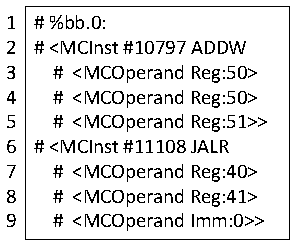
\includegraphics[scale=1.0]{image/MCLayer.pdf}
    \caption{MCLayer}
    \label{fig:MCLayer}
\end{figure}